\documentclass[compsoc,conference,a4paper,10pt,times]{IEEEtran}
\IEEEoverridecommandlockouts
\usepackage{cite}
\usepackage{amsmath,amssymb,amsfonts}
\usepackage{algorithmic}
\usepackage{graphicx}
\usepackage{textcomp}
\usepackage{bmpsize}
\usepackage{xcolor}
\usepackage{lipsum}
\usepackage{fancyvrb}
\usepackage[colorlinks=true,urlcolor=black]{hyperref}
\def\BibTeX{{\rm B\kern-.05em{\sc i\kern-.025em b}\kern-.08em
    T\kern-.1667em\lower.7ex\hbox{E}\kern-.125emX}}
\begin{document}

\title{Discreet Log Contracts Channels and Integration in the Lightning Network}

\author{\IEEEauthorblockN{Ichiro Kuwahara}
\IEEEauthorblockA{\textit{Crypto Garage} \\
Tokyo, Japan \\
kuwahara@cryptogarage.co.jp}
\and
\IEEEauthorblockN{Thibaut Le Guilly}
\IEEEauthorblockA{\textit{Crypto Garage} \\
Tokyo, Japan \\
thibaut@cryptogarage.co.jp}
\and
\IEEEauthorblockN{Takatoshi Nakagawa}
\IEEEauthorblockA{\textit{DG Lab} \\
Tokyo, Japan \\
nakagat@gmail.com}
}

\maketitle

\begin{abstract}
Contracts established on a blockchain remove the need for intermediary third parties, but usually require external data to decide on an outcome, provided by a so-called oracle.
Discreet Log Contracts (DLC) enable establishing such contracts directly on the Bitcoin blockchain without direct interaction with an oracle, increasing the privacy of the contracting parties.
Using the Bitcoin blockchain however also means hitting the scalability issues that are inherent to it.
To solve this issue, we propose a construction for establishing DLC off-chain through channels enabling the execution of consecutive contracts requiring only interaction with the blockchain during the setup and closing phases, similar to the functioning of the Lightning Network.
We provide an analysis of the construction to ensure its security, and then describe how DLC channels could be integrated in parallel to Lightning Network channels making them easier to use and enabling reuse of the Lightning Network's infrastructure.
\end{abstract}

\begin{IEEEkeywords}
Bitcoin, smart contract, payment channels
\end{IEEEkeywords}

\section{Introduction}
More than ten years after the writing of the Bitcoin white paper \cite{nakamoto2009bitcoin}, the Bitcoin blockchain is not only used as a way to transfer value, but also to establish financial contracts in a decentralized way.
These contracts can be specified using a simple scripting language (called Script in Bitcoin) that describes the spending conditions in a transaction.
They however usually rely on external data, such as a currency exchange rate, that is not directly available within the execution environment of the scripts.
To work around this limitation, a solution is to use oracles~\cite{ellis2017chainlink}, which provide such information in a format that can be used within a script's execution environment (usually in the form of a digital signature).
While putting a minimum amount of trust into oracles is unavoidable (assuming that they will not collude with one of the party in the contract), having the parties requesting data to them leaks the existence of the contract.

Discreet Log Contracts (DLC) \cite{dryja2017discreet} aim to solve this issue.
They enable two parties who do not trust each others to establish financial contracts directly on the Bitcoin blockchain without requiring direct interaction with an oracle.
This indirect interaction increases the privacy of the contracting parties as the oracle need not be aware of the contract’s existence.
DLC are also peer to peer contracts, in that they don't require any intermediate party to be established.
As an example, with DLC, futures and forward contracts can be established between two parties without having to put any of the funds in the custody of a cryptocurrency exchange.
However, as DLC are settled  on the Bitcoin blockchain, the settlement time as well as the fees that need to be paid to the miners can limit its scalability~\cite{decker2016scalability}. 
This puts DLC at a disadvantage compared to centralized solutions.

A common solution to these limitations is to make use of second layer protocols~\cite{gudgeon2020sok}, that enable the transfer of assets between parties outside of the blockchain (thus often called off-chain protocols), while still taking advantage of its security properties. 
Payment channels, and in particular the Lightning Network~\cite{poon2016bitcoin}, is currently one of the most widely used layer two solution.
We recall the building blocks of payment channels, as well as the functioning of DLC in Section~\ref{sec:prel}.
Inspired by payment channels, we present in Section~\ref{offdlc} a construction for establishing DLC channels, enabling the execution of consecutive contracts requiring interaction with the blockchain only during the setup and closing phases.

In order to implement these channels, a lot of work has to be done at multiple layers.
At the network level, the creation of a peer to peer network is a tedious task.
At the application level, monitoring of the blockchain for the broadcast of transactions from revoked states, as well as ensuring that liquidity is available in the channels are non trivial issues to be solved.
Fortunately, solutions have already been proposed in the context of the Lightning Network.
Having the ability for DLC channels to be embedded into the Lightning Network infrastructure would thus be highly beneficial.
Section~\ref{lninte} describes an approach to achieve this.

While the constructions presented in this paper have to the best of our knowledge not been proposed before, they draw inspiration from past and related work that we discuss in Section~\ref{related}.
We finally conclude and provide directions for further work in Section~\ref{conclusion}.
\section{Preliminaries}\label{sec:prel}

This section introduces the basic building blocks of payment channels as well as the original concept of DLC.

\subsection{Transactions}

In Bitcoin a transaction consists of a number of inputs and outputs.
Each output includes a script which specifies under which conditions the ownership of the value contained inside it can be transferred.
Each input refers to a previous output, and needs to provide arguments to satisfy its spending conditions.
Common examples are outputs checking for a digital signature from a specific private key, or requiring signatures from \emph{m} out of \emph{n} possible keys.
Outputs can also contain multiple spending conditions, or spending paths (for example one requiring a single signature, and another one requiring two) that can be created using \Verb_IF/ELSE_ statements.

\subsection{Payment channels}

Payment channels are currently among the most popular solutions to increasing the scalability of blockchain systems.
The concept of payment channels usually revolves around broadcasting a limited number of transactions on the blockchain (called \emph{on-chain} transactions), while enabling a much larger number of transactions to occur.
This can be securely achieved by having two parties exchange transactions and digital signatures in such a way that it is always possible for both of them to enforce the latest state of the channel (the balance between both parties) by broadcasting a transaction \emph{on-chain}, as well as to recover their funds in case their counter party broadcast an outdated state.
A basic assumption for payment channel is that both parties must be watching the blockchain for inclusion of stale transactions, or at least delegate this task to watchtowers~\cite{khabbazian2019}.

\subsection{Transaction revocation}\label{sec:trrev}

In order to protect the parties from the broadcast of an outdated state of the channel, the Lightning Network uses a transaction revocation mechanism.
It works by having both parties hold a different transaction with the same output values, but where the output paying them contains two spending paths:
* The first one requires a signature from a \emph{revocation key},
* The second one requires a signature from the party that holds it, but can only be spent after a certain amount of time has elapsed (using the \Verb_CHECKSEQUENCEVERIFY_ opcode~\cite{csv}).

A party can revoke a transaction by revealing the private key for the first spending path.
If this transaction was to be broadcast \emph{on-chain} in the future, the counter party has a certain amount of time to use the revocation key to claim the funds from the output.
Of course the parties should never reveal their signatures for \emph{their} revokable transactions, as it could allow their counter party to steal their fund if they also know the revocation key.

Note that the protocols and mechanisms for transactions and key exchanges are kept simple in this paper for the purpose of explanation, but the interested reader can refer to the Lightning Network specifications~(\cite{bolt2, bolt3}) for examples of how it can be done in practice.

\subsection{Discreet Log Contracts}\label{basedlc}
DLC were proposed to enable two parties to enter into a financial contract using Bitcoin transactions and an oracle, but without requiring direct interaction with the oracle, thus leaving a “discreet log”.
In other words, the parties do not have to inform the oracle of the contract being established.
This is achieved through a peculiar use of Schnorr signatures~\cite{schnorr1989efficient} that is described in detail in~\cite{dryja2017discreet}.

The second important property of DLC is that they don’t require trust between the parties, and only minimal trust to the oracle (essentially that it does not collude with one of the party).
This is achieved through the use of specially crafted Bitcoin transactions that we recall in this section.
The transaction flow is illustrated in Figure~\ref{fig:basedlc}.

\begin{figure}
  \centering
  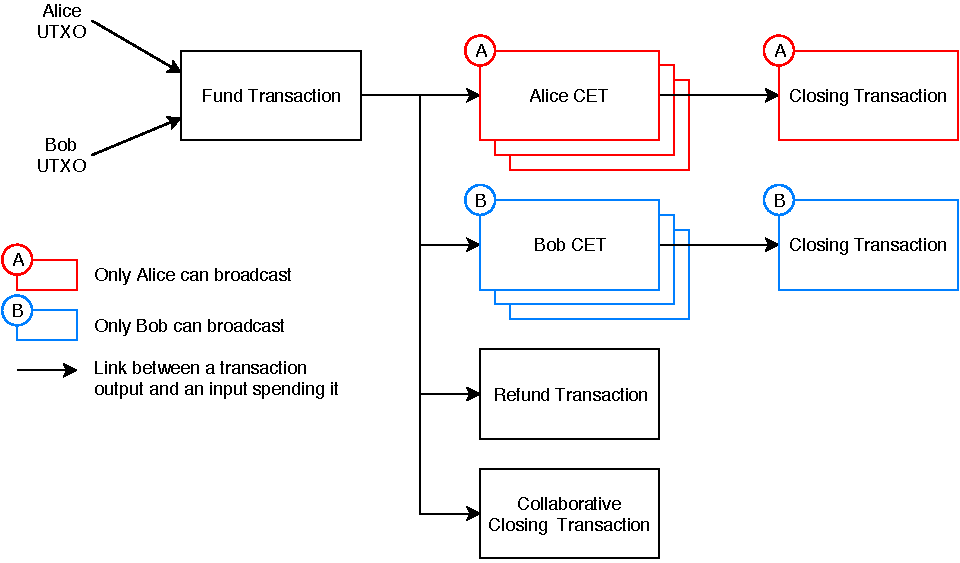
\includegraphics[width=\columnwidth]{Figures/BaseDlc.pdf}
  \caption{Illustration of the on-chain DLC transaction flow. Both parties lock their collaterals in the fund transaction, and can exercise the outcome of the contract through their CETs. Alternatively, the parties can agree to close the contract collaboratively, and if the oracle fails to produce a signature, they can recover their collaterals with the refund transaction.}
  \label{fig:basedlc}
\end{figure}

\subsection{Fund transaction}
The first transaction that makes up a DLC is the fund transaction.
This transaction takes a number of inputs coming from each of the parties UTXOs and locks the collateral of each party into a multi-signature script, requiring a signature from both parties to be unlocked.
It can also include change outputs when the sum of one of the party’s input UTXOs is greater than the desired contract collateral.
The output script for the multi-signature output of the fund transaction is detailed in Script~\ref{script:fundtx}.

\subsection{Refund Transaction}
The refund transaction is one of the transactions that can be used to spend from the fund transaction, and simply returns the collateral posted by each party.
It is intended to be used only in the case where the oracle does not publish a signature for the event on which the DLC is based on.
For that reason, it is time locked, meaning that it cannot be included in the blockchain before a certain timestamp, that should be set to after the maturity date of the contract.

\subsection{Contract Execution Transactions}
A contract execution transaction (CET) is the second type of transaction that can spend from the fund transaction.
It encodes a possible outcome of the contract, meaning that there must be as many CETs as possible outcomes of the contract.
Both parties hold a different set of CETs, each including two outputs.

The first output of a CET consists of a script that enables either the party broadcasting it to spend it by using a combination of its private key and the oracle signature, or their counter party after a certain time has elapsed after the transaction was included in the blockchain (using the Check Sequence Verify op-code \cite{csv}, the script is detailed in Script~\ref{script:cet}).
This ensures that if one of the parties was to broadcast a CET that did not correspond to the outcome revealed by the oracle, they would lose their fund (this is somewhat similar to the transaction revocation concept discussed in Section~\ref{sec:trrev}).

The second output can be spent directly by the counter party of the broadcaster.

\subsection{Closing Transaction}
The closing transaction is used by the broadcaster of a CET to retrieve the funds locked in the first output.
It satisfies the script of the first CET output by providing a signature that is created using a combination of the spender’s private key and the oracle signature.

\subsection{Signing Order}
In order to guarantee that both parties can always either recover their funds or execute the contract, the transactions need to be signed in a specific order. 

First, the signatures for the CETs and the refund transaction are exchanged.
As the fund transaction they spend from has not been signed yet, they cannot be used.

The signatures for the fund transaction are then exchanged.
Note that as this exchange happens non atomically, one of the parties will obtain the other party's signature first.
This gives them a “free option”, in the sense that they can choose to execute the contract only in the event that the outcome is favorable to them.
However, if the counter party does not receive the expected signature, they can choose to spend their UTXOs included in the fund transaction, rendering it invalid, and thus cancelling the contract.

\subsection{Collaborative Closing}

Given the above described transactions, executing a DLC requires broadcasting three transactions: the fund transaction, a CET and a closing transaction.
However, once the Oracle has published the outcome, the parties can decide to create a collaborative closing transaction with the same output amounts as the CET for the announced outcome.
This reduces the number of required transactions to two.
If the parties would like to re-establish a contract after maturity, another two transactions will have to be broadcast \emph{on-chain}.

\section{DLC Channels}\label{offdlc}

In this section, we first describe a naive approach to establishing and updating a DLC contract off-chain, and show why it fails.
We then present our solution to securely do it.

\subsection{A straw-man proposal}\label{strawman}

A simple approach to establish off-chain DLC is to make CETs and the refund transaction revocable.
We assume two parties, Alice and Bob, want to create a DLC channel, to be able to establish multiple consecutive contracts.
The protocol would be as follow:
\begin{enumerate}
  \item Alice and Bob create all transactions and exchange signatures according to the \emph{regular} DLC protocol,
  \item Bob broadcasts the fund transaction,
  \item After contract maturity, they create a new set of CETs and a new refund transaction representing the new contract to establish,
  \item Alice sends to Bob her signatures for the new CETs and refund transaction,
  \item Bob sends to Alice his signatures for the new transactions,
  \item\label{problem} Alice sends to Bob her revocation key, \emph{revoking} her previous CETs and refund transaction,
  \item Bob sends to Alice his revocation key for the previous DLC transactions.
\end{enumerate}

At the end of this protocol, both Alice and Bob have the set of signed transactions for the second DLC, and the transactions for the previous one are revoked.
However, there is an issue at step~\ref{problem}.
After sending her revocation secret to Bob, Alice cannot anymore enforce the result from the first contract.
However, as Bob has not yet revealed his secret, he still has the ability to do so, in addition to having the ability to enforce the second one.
If Bob is dishonest, he could thus choose not to reveal his revocation key, and wait until just before the maturity of the second contract to execute the one that is most favorable to him (he could also potentially use the previous refund transaction if the time lock expired).
Note that the Lightning Network does not suffer from this issue, as when updating a channel, the payer should reveal their secret first as the update will be unfavorable to them.

In order to solve this issue, we introduce two new types of transactions in the protocol.

\subsection{Update transaction}
The first new transaction is the update transaction.
It is similar in structure to the \emph{commitment} transaction in the Lightning Network, taking as input the multi-signature output of the fund transaction, and containing two outputs, representing the current balance of each party in the channel.
Each party holds a different update transaction, in order to enable their revocation.
The first output contains three different spending paths (the script for this output is detailed in Script~\ref{script:updatetx1}). 
We describe here the required arguments for the three paths of the first output of the transaction held by Alice:
\begin{enumerate}
  \item A signature from Alice's revocation key, 
  \item A signature from both Alice and Bob, plus a time delay (CSV) $d_1$,
  \item A signature from Alice, plus a time delay (CSV) $d_2$.
\end{enumerate}

The second output contains two different spending paths (the script is detailed in Script~\ref{script:updatetx2}), requiring either:
\begin{enumerate}
  \item A signature from both Alice and Bob,
  \item A signature from Bob, plus a time delay (CSV) $d_2$.
\end{enumerate}

Note that it is necessary that $d_1 < d_2$ as will become clear in the description of the protocol in Section~\ref{offdlcproto}.
The version held by Bob is similar, with Bob and Alice's signatures reversed.

\subsection{Buffer transaction}
A buffer transaction consumes both outputs of an update transaction, using the multi-signature paths.
It combines the value of these inputs into a single output, requiring both Alice and Bob signatures to be unlocked (the script is detailed in Script~\ref{script:buffertx}).

\subsection{Offchain DLC protocol}\label{offdlcproto}
Having these two new types of transactions, we can describe the protocol for establishing and updating a DLC channel.
The transaction flow is illustrated in Figure~\ref{fig:full}.

\begin{figure*}
  \centering
  \includegraphics[width=\textwidth]{Figures/fullOffChainDLC.pdf}
  \caption{Illustration of the transaction flow for the establishment and update of a DLC channel. The addition of the update and buffer transactions enables both parties to safely re-enter in a contract after a previous one has expired.}
  \label{fig:full}
\end{figure*}

\subsubsection{Establishment}
The establishment of a DLC channel is similar to that of an \emph{on-chain} DLC.
We make use of the two new types of transaction for consistency across the protocol steps, but note that at this stage they are not strictly required (one could instead make the CETs and the refund transaction revokable for this initial contract, as long as the update and buffer transactions are used for establishing the second one).
In the following, we assume that the terms of the contract are already agreed upon between the participants:
\begin{enumerate}
  \item Alice sends to Bob the set of UTXOs she wants to use to fund the channel, a public key for later revocation, as well as a set of public keys to be used in the transactions,
  \item Bob selects a set of UTXOs, and using the information received from Alice constructs the transactions and generates signatures for them,
  \item Bob sends back his set of UTXOs and public keys, as well as his signatures for all transactions except for the fund transaction and \emph{his} update transaction,
  \item Alice creates the transactions and signatures, and sends the signatures to Bob (except for \emph{her} update transaction),
  \item Bob adds the signatures to the fund transaction and broadcasts it.
\end{enumerate}

As in regular DLC, parties are ensured that their funds can always be unlocked by signing the fund transaction last.
Note that both parties should validate the signatures they receive.

\subsubsection{Update}

At contract maturity, once the oracle has released a signature, Alice and Bob can decide to create a mutual closing transaction to terminate the contract, or if one party is uncooperative, the other party can broadcast the update, buffer, appropriate CET and closing transactions.
We assume here that instead they wish to enter in another contract, and have already agreed on the terms.
They can then use the following protocol:
\begin{enumerate}
  \item Alice and Bob generate the set of transactions (update, buffer, CETs and refund) for the new contract, with the update transactions having output values equal to the outcome of the previous contract,
  \item \label{a1} Alice sends her signatures for Bob's update transaction, all CETs and the refund transactions,
  \item \label{b1} Bob sends his signatures for Alice's update transaction, all CETs, the refund transactions, as well as the revocation key for his previous update transaction,
  \item \label{a2} Alice sends the revocation key for her previous update transaction, as well as the signature for her buffer transaction,
  \item \label{b2} Bob sends his signatures for both buffer transactions.
  \item \label{a3} Alice sends her signature for Bob's buffer transaction.
\end{enumerate}

We go through the different steps of this protocol to analyze the possible actions of both participants after each step.

\paragraph{Step \ref{a1}}: Bob obtained Alice's signature for his update transaction, giving him the ability to broadcast it.
However, as he does not have Alice's signature for the following buffer transaction, he would only be able to use the third script path returning him the same amount as decided by the outcome of the previous contract, after expiration of the time lock.
Alice would also recover the same amount as she was awarded by the outcome of the previous contract.
Given the information held by each party at this stage, Bob's update transaction resembles a mutual closing transaction, with a time delay.
Alice on her side still has the possibility of unilaterally closing the previous contract would Bob stop cooperating.

\paragraph{Step \ref{b1}}: Bob has revealed the revocation key for his previous update transaction, and can thus no longer broadcast it safely without risking to be penalized.
But since he has the ability to recover his due funds with the last update transaction, he still can exit the channel would Alice stop cooperating.
Alice also obtained the ability to broadcast her update transaction (but not the following buffer transaction).

\paragraph{Step \ref{a2}}: Alice revoked her previous update transaction, and Bob has the ability to broadcast Alice's buffer transactions.
That means that if Alice were to broadcast her fund transaction, Bob can force Alice to honor the contract.
While Alice doesn't yet have the same ability, broadcast of Bob's update transaction would only lead to settling the channel on the previous contract's outcome.
If Bob were to stop collaborating at this point, Alice can broadcast her update transaction to either force Bob to broadcast her buffer transaction and enter in the contract, or exit the contract at the latest state.

\paragraph{Step \ref{b2}}: Alice obtained the ability to broadcast both buffer transactions, either for unilaterally closing the contract after maturity using the path starting with her update transaction, or for forcing Bob to honor the contract were he to broadcast his update transaction before the term.

\paragraph{Step \ref{a3}}: Bob now also has the ability to broadcast all transactions, except for Alice's update transaction.

\subsection{Comparison with on-chain protocol}

Compared with the on-chain version, we note that the off-chain protocol leads to a larger number of transactions to be broadcast in the case of a unilateral close (5 compared to 3).
However, unilateral closes are expected to be an exception, and cooperative closes still only require two transactions to be broadcast.
In addition, the off-chain protocol enables the execution of an unlimited number of contracts, and apart from the update and buffer transactions, the other transactions are the same as the on-chain version, meaning that implementations can reuse the code from the off-chain version.

\section{Integration with the Lightning Network}\label{lninte}

While having the protocol presented in Section~\ref{offdlcproto} theoretically enables the creation of DLC channels, implementing all the necessary infrastructure would require a lot of additional work.
A lot of this work has already been carried on by the many researchers and developers who have contributed to the development of the Lightning Network.
Leveraging this work, and new or on-going research such as channel splicing, sub-marine swaps or channel factories~\cite{burchert2018scalable} for the creation of DLC channels would thus reduce the required effort.

In addition, if two parties who already have an established Lightning Network channel open with each others wished to create a DLC channel, it would be impractical and wasteful for them to have to broadcast another fund transaction.
Another issue arises if the parties wish to establish several contracts concurrently, as this would require opening several channels between the two parties.
Finally, as two parties participate in consecutive contracts within a DLC channel, it might become imbalanced, preventing further contracts to take place.

In this section, we propose a way to integrate DLC channels within the Lightning Network to enable:
* Reusing the Lightning Network infrastructure for peer discovery, channel funding, as well as recent innovations such as channel factories or splicing,
* the two parties of a lightning channel to establish multiple DLC channels in parallel to the lightning one, reusing the same fund transaction,
* the reallocation of funds between a lightning channel and DLC channels.

An illustration of the transactions for the integration of a single DLC channel with a lightning one is given in Figure~\ref{fig:lnin}.

\begin{figure*}
  \centering
  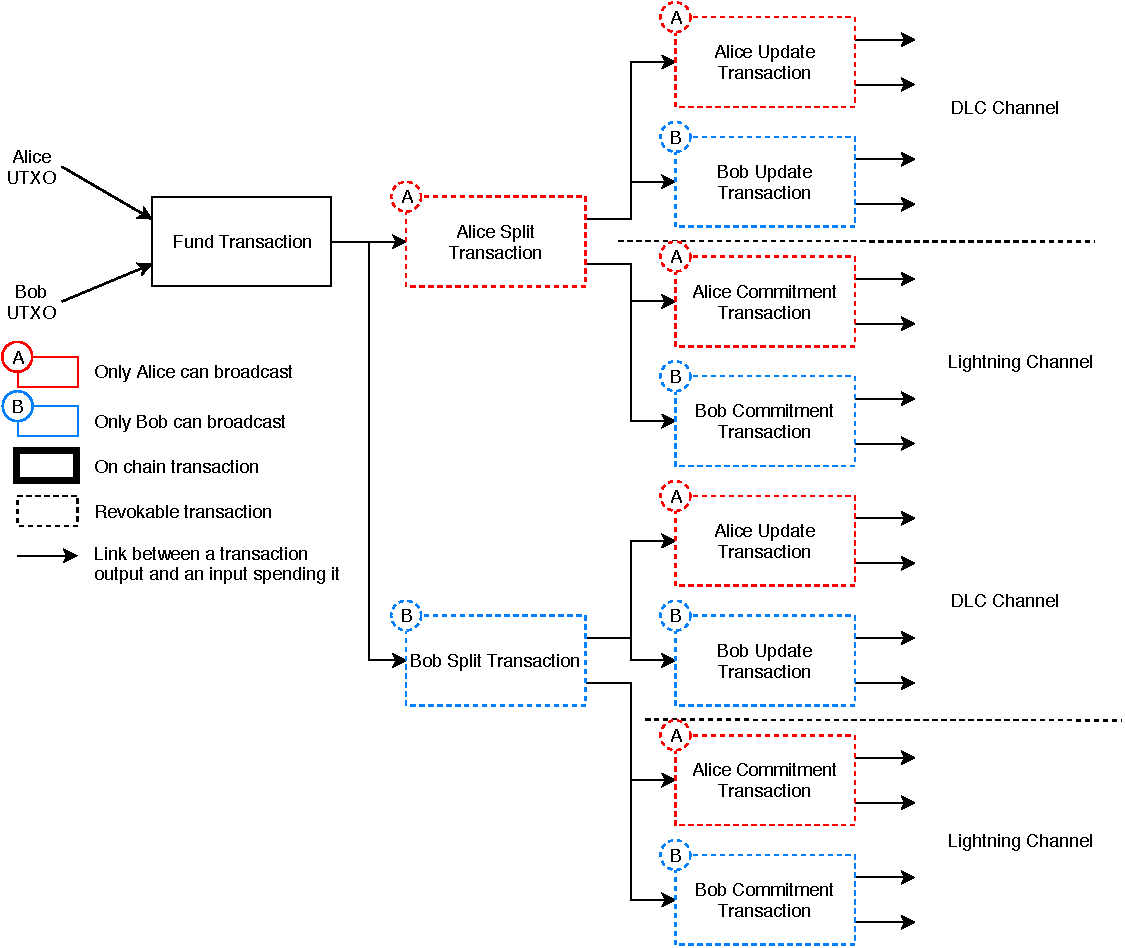
\includegraphics[width=\textwidth]{Figures/LightningIntegration.pdf}
  \caption{Illustration of the transaction construction for splitting a channel into a DLC and lightning one.}
  \label{fig:lnin}
\end{figure*}

\subsection{Split transaction}

To divide the allocation of funds from the fund transaction to both the lightning and DLC channels, we introduce a \emph{split transaction}.
This transaction contains multiple outputs, one for the funding of the lightning channel, and one for the funding of each of the DLC channels, each with a revocation path and a multi signature path (detailed in Script~\ref{script:splittx}).
Due to the revocation paths, each party needs to hold a different version of a split transaction.

\subsection{Channel splitting}

Here we assume that a dual funded lightning channel already exists between Alice and Bob, that they wish to establish a single DLC channel in parallel (the protocol generalizes to multiple ones), and that they have agreed on how much funds to allocate to each channel.
The protocol for a channel split is as follow:
\begin{enumerate}
  \item Alice sends signatures for Bob's update (for the DLC channel), commitment (for the lightning channel) and split transactions,
  \item Bob sends signatures for Alice's update, commitment and split transactions, as well as the secret for his previous commitment transaction,
  \item Alice sends the secret to her previous commitment transaction,
  \item Alice and Bob follow a protocol similar to presented in Section~\ref{offdlcproto} to finish the establishment of the DLC channel, with the difference of having to handle four sets of transactions instead of two (due to the asymmetry of the \emph{split transaction}).
\end{enumerate}

Subsequently, both channels can be updated independently.

If Alice and Bob wish to re-balance the funds between the lightning and DLC channels, they can follow a similar protocol, but revoke the split transactions instead of the initial commitment transactions of the lightning channel.

Finally, they can also close the DLC channel and return to a simple lightning channel by creating new commitment transactions allocating the sums of the funds of each party in each channel before revoking the \emph{split transaction}.

\subsection{Discussion}\label{discuss}

One of the main drawback of our proposed split channel design, is the larger amount of transactions to keep track of.
This increases the complexity of the system as well as the burden for watchtowers~\cite{khabbazian2019}.

Another approach to integrate DLC channels together with lightning channel would be to use an extra output in the lightning channel's commitment transaction, that can be used as a funding input to a DLC.
This was proposed by Bedn\'ar and Pickhardt~\cite{bednar2019}.
While it does effectively reduce the number of transactions, it also means that for each update of the lightning channel, all the transactions for the DLC need to be reconstructed, signed and exchanged.
The update of each channel also becomes dependent on the state of the other channel, potentially leading to concurrency issues.
We thus believe that the extra cost induced by the split of the channel is compensated by a better separation between the two channels and the ability to update them independently.

We also note that this splitting approach, while designed in the context of allowing DLC channels within the Lightning network, could also be used to integrate other types of channel relying on a fund transaction.
\section{Related Work}\label{related}

As already discussed in Section \ref{discuss}, Bedn\'ar and Pickhardt \cite{bednar2019} previously proposed DLC channels embedded in the Lightning Network.
Their construction works by adding an extra output to the commitment transaction of a lightning channel, which is used as the funding for a DLC.
One of the disadvantage of this approach is the complex interaction between the DLC and lightning channels.
They also mention splitting a channel into a DLC and lightning one by extending the peer protocol of the Lightning Network, but details on how this would be achieved are not given making it difficult to compare with our proposed approach.
Finally, the authors also mention the possibility to improve the construction if Bitcoin introduces the \texttt{SIGHASH\_NOINPUT} signature hash, as well as using channel factories.
\texttt{SIGHASH\_NOINPUT} would indeed allow for much simpler and more general constructions similar to the eltoo protocol~\cite{decker2018eltoo}.

Channel factories \cite{burchert2018scalable} could indeed prove useful to make it easier to create DLC channels as well as increase the scalability for channel setup.

While we chose the penalty model of the Lightning Network as a basis for the DLC channel construction, in part due to the desire of enabling integration within it, the model of micro-payment channels~\cite{decker2015fast} could also be a viable approach, potentially reducing the asymmetry of the transactions.

\section{Conclusion and Future Work}\label{conclusion}

In this paper we presented a construction for the establishment of DLC channels.
These channels enable the execution of multiple consecutive contracts between two parties, while requiring the same amount of on-chain transactions as regular DLC in the best case, and two more transactions in the non-cooperative case.
We then proposed an approach to integrate DLC channels within the Lightning Network, to reuse infrastructure and technological advances.
This approach could also be used to integrate other types of protocols within the Lightning Network, as long as they use a fund transaction.
We plan on implementing this integration in the near future, with a goal of enabling Lightning Network users to enter in various contracts with the parties with which they have a channel open.

Another important part of DLC not touched upon in this paper is the communication between the oracle and the contracting parties.
Here again, leveraging the existing Lightning Network peer to peer network layer could reduce the amount of required work.
Communication through the Lightning Network channels could also be considered, enabling payments to oracles.

Potential upgrades to the Bitcoin protocol will also have an impact on how DLC channels can be implemented.
Firstly, the native support of Schnorr signatures will enable scriptless script versions of DLC.
This would remove the necessity of a penalty mechanism, as well as enabling contracts between three or more parties to be established.
Secondly, the addition of a signature hash type such as \texttt{SIGHASH\_NOINPUT} would greatly reduce the complexity of the channel construction.
We will thus be monitoring these advances closely to integrate them in the planned implementation of DLC channels when they become available.

Finally, while the analysis of the protocols presented in this paper gives us confidence in their correctness, we would like in future work to leverage the advances in formal analysis applied to Bitcoin~\cite{bartoletti2018bitml} to formally verify them.


\bibliography{references}{}
\bibliographystyle{plain}

\appendices

\newtheorem{script}{Script}

\section{Transaction scripts}\label{append1}

For completeness, this appendix lists the scripts for the transactions that are used in the establishment and update of DLC channels.

\begin{script}[Fund transaction output script]\label{script:fundtx} \\
\begin{Verbatim}[samepage=true]
OP_2 
<alice public key> 
<bob   public key> 
OP_2 
OP_CHECKMULTISIG 
\end{Verbatim}
\end{script}

\begin{script}[Script for the first output of an update transaction]\label{script:updatetx1}\\
\begin{Verbatim}[samepage=true]
OP_IF
    <delay 1>
    OP_CHECKSEQUENCEVERIFY
    OP_DROP
    OP_2
        <alice public key>
        <bob   public key>
    OP_2
    OP_CHECKMULTISIG
OP_ELSE
    OP_IF
        <delay 2>
        OP_CHECKSEQUENCEVERIFY
        OP_DROP
        <alice/bob public key>
    OP_ELSE
        <alice/bob revocation public key>
    OP_ENDIF
    OP_CHECKSIG
OP_ENDIF
\end{Verbatim}
Note that \Verb _delay 1_ must be less than \Verb _delay 2_.
\end{script}

\begin{script}[Script for the second output of an update transaction]\label{script:updatetx2}\\
\begin{Verbatim}[samepage=true]
OP_IF
    OP_2
        <alice public key>
        <bob   public key>
    OP_2
    OP_CHECKMULTISIG
OP_ELSE
    <delay 2>
    OP_CHECKSEQUENCEVERIFY
    OP_DROP
    <alice/bob public key>
    OP_CHECKSIG
OP_ENDIF
\end{Verbatim}
Note that \Verb _delay 2_ should be the same value as used in the first output.
\end{script}

\begin{script}[Buffer transaction output script]\label{script:buffertx}\\
\begin{Verbatim}[samepage=true]
OP_2
    <alice public key>
    <bob   public key>
OP_2
OP_CHECKMULTISIG
\end{Verbatim}
\end{script}

\begin{script}[Script for the first output of a CET]\label{script:cet}\\
\begin{Verbatim}[samepage=true]
OP_IF
    <alice/bob public key>
      + <oracle message public key>
OP_ELSE
    <delay 3>
    OP_CHECKSEQUENCEVERIFY
    OP_DROP
    <bob/alice public key>
OP_ENDIF
OP_CHECKSIG
\end{Verbatim}
Note that the \Verb _+_ operator represents elliptic curve point addition.
\end{script}

\begin{script}[Output script of a split transaction]~\label{script:splittx}\\
\begin{Verbatim}[samepage=true]
OP_IF
    <alice/bob revocation public key>
OP_ELSE
    <delay>
    OP_CHECKSEQUENCEVERIFY
    OP_DROP
    <alice/bob public key>
OP_ENDIF
OP_CHECKSIG
\end{Verbatim}
\end{script}

\end{document}
